\documentclass[11pt]{article}
\usepackage[left=1in ,bottom=1in ,left = 1in, right = 1in]{geometry}
\usepackage{graphicx}
\begin{document}
\title{\begin{huge}AVILASH MOHANTY\end{huge}}
\maketitle

\begin{flushleft}
$\#$420 BH-II,GGSIPU, 
\hfill{Contact: (+91)9560372680}\\
NEW DELHI, 
\hfill{e-mail\_id: avilashmohanty1920@gmail.com}\\
New Delhi-110078

\end{flushleft}

\begin{flushright}
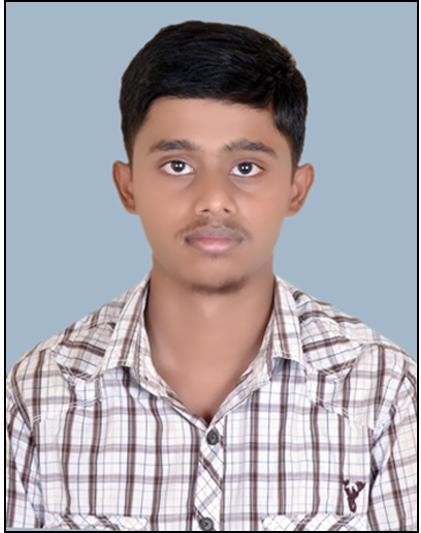
\includegraphics [scale=0.25]{picture.jpg}
\end{flushright}

\begin{flushleft}
		\noindent {\Large \bf Objective} 
		\vskip .2cm
		\hspace{.2in}
		  To improve my technical skills
	\end{flushleft}
	
\begin{flushleft}

\Large
\textbf{Education }
\vspace{0.5in}
{
%\begin{centre}
\small
\begin{tabular}{|c|c|c|c|c| }

\hline
\small
Degree/Class & School/College & University/Board & Year &  $\%$age/CGPA\\ 
\hline
\small 10th & KV High Grounds,Chandigarh & CBSE & 2012 & CGPA 10.0\\
\hline

\small 12th & KV Arjangarh,New Delhi & CBSE & 2014 & 89\% \\
\hline

\small B.Tech ECE  & University School of Information and Communication technology,New Delhi & GGSIPU & 2014-2017 & 94.6\% \\
\hline

\end{tabular}
%\end{centre}
}
\end{flushleft}

\begin{flushleft}
\vspace{0.1in}
{\Large \bf Projects} 
\begin{enumerate}
\vspace{0pt}	                                  		\addtolength{\itemindent}{1in}	                                  \item  E-yantra robotics hazardous waste disposal theme in E-Yantra'2015-16.

	                                  		\item Working on a QuadCopter project for Infox '16  \\
	                                  		\hspace{1.3in}
\end{enumerate}
\end{flushleft}
	                                  

\end{document}

 